\chapter{Architecture}
\label{chapter:arch}

The architecture of the project involves 3 layers:
\begin{itemize}
\item \textbf{Eos} - A low level layer that handles effects and attributes using DOGMA. This layer should be very abstract and not care about EVE at all. This is already implemented as part of a community effort.
\item \textbf{Raven} - A middle layer that augments the first one by exposing methods that return high-level information that only makes sense in the world of EVE Online.
\item \textbf{Tengu} - A service layer and a GUI, that will serve visual information to users and handle their requests.
\end{itemize}

\begin{figure}[h]
\centering
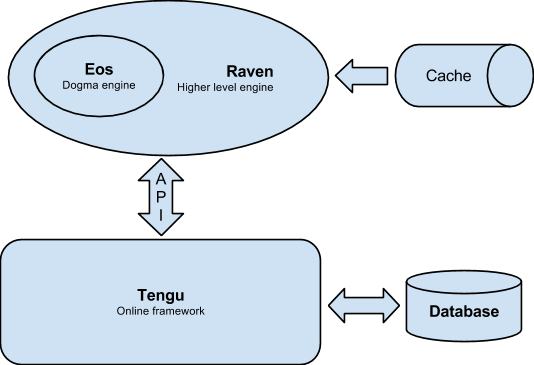
\includegraphics[width=0.7\linewidth]{src/img/arch}
\caption{Architecture of the project}
\label{fig:arch}
\end{figure}

The first layer, represented by Eos, should be as decoupled from EVE as possible. Apart from knowing the structure of the database, Eos will only care about abstract entities. It will not differentiate between a weapon module and a defensive one. They will both be represented as modules that have certain effects that can be applied to certain targets.

This makes for a robust and flexible engine that can easily be adapted and maintained. If the game changes at some point, Eos should theoretically still work.

Raven, the middle layer, will extend Eos by taking all those low level attributes and outputting information that means something in the game of EVE Online: things like align time, capacitor stability, damage per second and the amount of incoming damage it can sustain. Raven will inherit Eos and will add its new methods on top of it. It will be released under an open-source license so other players can contribute to it, making it faster and more accurate.

The service layer will handle the creation and sharing of fits. User management will also be handled by this layer, along with the API that allows 3rd party developers to make use of the functionalities exposed by the middle layer. The GUI will tie all these things together and present them in a way that is both beautiful and intuitive.

Tengu will allow limitless potential for creating fits with any item in the game and sharing them with other players. Tengu will provide a sleek interface that will resemble what players have been used to ingame. It will be made available to the public, but it will be closed-source as to not expose any critical security features that might be exploited.

